\section{Prediction problem formulation}

Based on the literature review in Chapter 2, the system requirements defined in Chapter 3, the database validation in Chapter 7, and the exploratory data analysis presented in the previous chapter, the machine learning prediction problem can now be formally defined. Earlier chapters established the limitations of existing impact-based forecasting systems and identified the characteristics of the constructed drought impact database. These findings are used to define the spatial scale, forecasting horizon, and impact categories considered in the prediction task.

The objective is to predict the occurrence of multiple drought impacts for a given region and future time period. Each observation consists of a region $r$ at time $t$, represented by a feature vector:

\begin{equation}
\mathbf{x}_{r,t} =
[x_1,x_2,\ldots,x_p],
\end{equation} where $p$ represents the number of predictor variables describing the state of the region at time $t$. The prediction target is represented as a multi-label vector:

\begin{equation}
\mathbf{y}_{r,t+h} =
[y_1,y_2,\ldots,y_K],
\end{equation} where $K$ represents the number of impact classes considered in the prediction framework. Each element of the vector is defined as:

\begin{equation}
y_k =
\begin{cases}
1, & \text{if impact class } k \text{ occurs in region } r \text{ at time } t+h,\\
0, & \text{otherwise.}
\end{cases}
\end{equation} The objective of the machine learning model is to estimate future drought impact occurrences based on the available predictor variables. This can be formulated as:

\begin{equation}
\hat{\mathbf{y}}_{r,t+h}=f(\mathbf{x}_{r,t}),
\end{equation} where $f$ represents the trained machine learning model, $\mathbf{x}_{r,t}$ represents the predictor variables describing region $r$ at time $t$, and $\hat{\mathbf{y}}_{r,t+h}$ represents the predicted impact occurrence vector for region $r$ at lead time $h$.



In this thesis, the general formulation above is specified based on the limitations and opportunities identified in previous chapters. The spatial unit $r$ is defined at the NUTS-3 regional level. This choice addresses a limitation identified in previous impact-based forecasting studies, where predictions were often performed at larger spatial scales, such as national, NUTS-1, or provincial levels. Although these larger spatial units reduce prediction difficulty by aggregating local variability, they provide limited information for regional decision making.

The forecasting horizon $h$ is defined as zero to three months, with particular focus on one-month-ahead predictions. This choice follows findings from previous studies, which indicate that predictive skill generally decreases as lead times increase and approaches random performance at longer forecasting horizons. The prediction period for training and testing will be from 2018-2025 based on the distrubtion shift after 2018 period. 

Finally, the prediction target consists of the ten most frequently occurring impact classes identified during the exploratory data analysis. Restricting the prediction task to these classes ensures that each predicted impact has sufficient historical observations for model training while maintaining the multi-impact structure of the database. Based on the observed frequency distribution, each selected impact class contains at least approximately 440 observations, providing a more reliable basis for machine learning compared to rare impact categories.

The predictor variables used as input to the model are defined in the following section.


\section{Predictor variables}

The predictor variables form the feature vector $\mathbf{x}_{r,t}$ and are selected based on previous literature, system requirements, and insights obtained from the drought impact database. The aim is to provide an initial feature space that represents the main processes through which drought conditions translate into impacts. The final predictor configuration is determined during the modelling phase using automated optimization methods.

The predictors are divided into three main categories. The first category consists of drought-related variables describing the current hydro-meteorological conditions. These include meteorological drought indicators such as SPI and SPEI at multiple accumulation periods, soil moisture anomalies, and consecutive dry day indicators. These variables are aggregated from spatial datasets to the NUTS-3 regional level.

The second category consists of static regional characteristics describing differences in exposure and vulnerability between regions. These variables include land cover, population characteristics, and other regional properties that may influence how strongly a region responds to drought conditions. Additional variables proposed from the exploratory analysis and expert consultation include soil composition and regional elevation, as these characteristics may influence water retention and local drought sensitivity.

The third category contains temporal variables that describe the temporal behaviour of drought impacts. These include seasonal variables, previous impact occurrences, and lagged impact information. These variables allow the model to capture recurring patterns and persistence in drought impacts.

Together, these predictor categories provide a broad representation of drought conditions, regional characteristics, and temporal dynamics. The final predictor set is selected during the automated modelling procedure described in the following section.

\begin{table}[h]
\centering
\small
\caption{Candidate predictor variables included in the initial feature space.}
\label{tab:predictor_space}
\begin{tabular}{p{3.5cm} p{10.5cm}}
\toprule
\textbf{Predictor category} & \textbf{Candidate variables} \\
\midrule

Hydro-meteorological variables &
Standardized Precipitation Index (SPI) at multiple accumulation 1-24 months, 
Standardized Precipitation Evapotranspiration Index (SPEI) at multiple accumulation 1-24 months, 
soil moisture anomalies, consecutive dry days (CDD)\\

Regional characteristics &
Land cover, population characteristics, soil composition, regional elevation \\

Temporal variables &
Seasonal variables, previous drought impact occurrences, and lagged impact information 
describing temporal persistence and recurring impact patterns \\

\bottomrule
\end{tabular}
\end{table}





\section{Model optimization and evaluation}

The objective of the modelling procedure is to identify a suitable combination of predictor variables and machine learning models for multi-label drought impact forecasting. Since multiple combinations of predictor variables, algorithms, and model configurations are possible, an automated optimization approach is used to efficiently identify high-performing model configurations.

The dataset is divided using a temporal evaluation strategy to reflect the objective of forecasting future drought impacts. Random splitting is avoided because drought impacts are strongly related to specific drought events, and observations close together in time may contain similar information. A temporal split provides a more realistic estimate of model performance when applied to future drought conditions.

The period from 2018 to 2023 is used as the model development period. This period contains multiple drought events (2018, 2019, and 2022) and is used for model training, predictor selection, and model optimization. Within this period, expanding-window temporal cross-validation is applied (Figure~\ref{fig:temporal_cv}). During each validation step, the model is trained using only data from previous years and validated on the subsequent year. This ensures that model selection is based on the ability to predict future periods rather than reconstruct historical observations.


\begin{figure}[h]
\centering
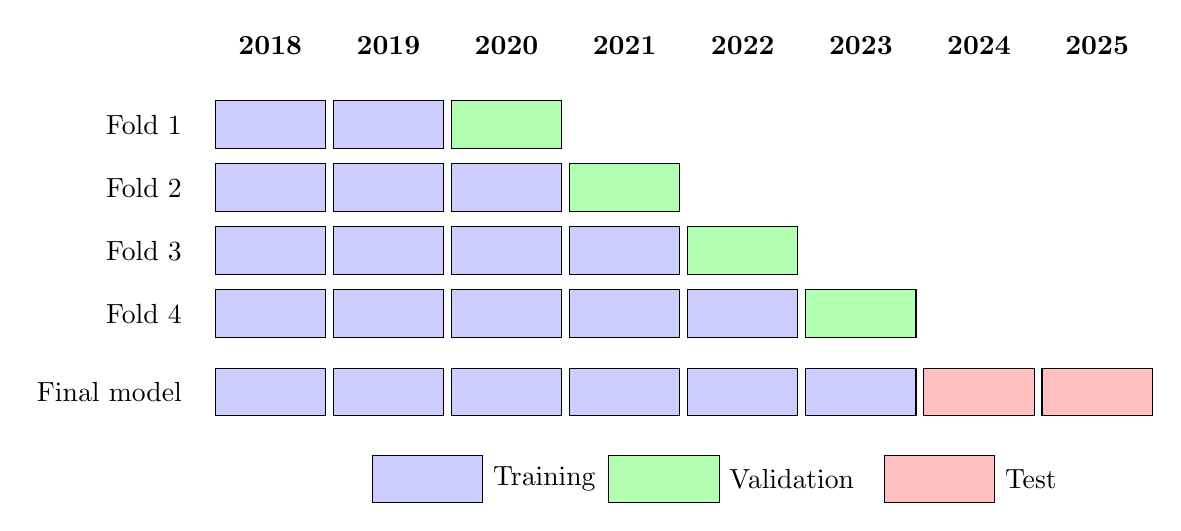
\begin{tikzpicture}[
    year/.style={draw, minimum width=1.4cm, minimum height=0.6cm},
    train/.style={year, fill=blue!20},
    valid/.style={year, fill=green!30},
    test/.style={year, fill=red!25}
]

% Year labels
\node at (0,3.5) {};
\foreach \x/\y in {0/2018,1.5/2019,3/2020,4.5/2021,6/2022,7.5/2023,9/2024,10.5/2025}
{
    \node at (\x,4) {\textbf{\y}};
}

% Fold 1
\node[left] at (-1,3) {Fold 1};
\node[train] at (0,3) {};
\node[train] at (1.5,3) {};
\node[valid] at (3,3) {};

% Fold 2
\node[left] at (-1,2.2) {Fold 2};
\node[train] at (0,2.2) {};
\node[train] at (1.5,2.2) {};
\node[train] at (3,2.2) {};
\node[valid] at (4.5,2.2) {};

% Fold 3
\node[left] at (-1,1.4) {Fold 3};
\node[train] at (0,1.4) {};
\node[train] at (1.5,1.4) {};
\node[train] at (3,1.4) {};
\node[train] at (4.5,1.4) {};
\node[valid] at (6,1.4) {};

% Fold 4
\node[left] at (-1,0.6) {Fold 4};
\node[train] at (0,0.6) {};
\node[train] at (1.5,0.6) {};
\node[train] at (3,0.6) {};
\node[train] at (4.5,0.6) {};
\node[train] at (6,0.6) {};
\node[valid] at (7.5,0.6) {};

% Final test
\node[left] at (-1,-0.4) {Final model};
\node[train] at (0,-0.4) {};
\node[train] at (1.5,-0.4) {};
\node[train] at (3,-0.4) {};
\node[train] at (4.5,-0.4) {};
\node[train] at (6,-0.4) {};
\node[train] at (7.5,-0.4) {};
\node[test] at (9,-0.4) {};
\node[test] at (10.5,-0.4) {};

% Legend
\node[train, label=right:Training] at (2,-1.5) {};
\node[valid, label=right:Validation] at (5,-1.5) {};
\node[test, label=right:Test] at (8.5,-1.5) {};

\end{tikzpicture}
\caption{Expanding-window temporal cross-validation used for model development. The final model is retrained on the complete development period (2018--2023) before evaluation on the independent test period (2024--2025).}
\label{fig:temporal_cv}
\end{figure}


Temporal cross-validation is chosen because drought impacts are expected to depend on conditions in previous years. For example, systems may be more or less vulnerable depending on antecedent soil moisture conditions or whether they have already been affected by previous drought impacts. Using an expanding temporal split therefore better reflects the real-world forecasting setting and avoids information leakage from future observations.


The period from 2024 to 2025 is reserved as an independent test period. These years are not used during model optimization and are only used for the final evaluation of the selected model. This provides an estimate of the expected model performance when applied to unseen future drought events. The test period includes one relatively normal year (2024) and one drought year (2025), allowing the model to be evaluated under contrasting hydroclimatic conditions.
The automated optimization procedure searches over the predefined search space shown in Table~\ref{tab:search_space}. The search space consists of candidate machine learning algorithms, predictor and model-specific hyperparameter ranges. Each candidate configuration is evaluated using the expanding-window temporal cross-validation procedure described above, and the configuration with the highest validation performance is selected for the final model.

\begin{table}[h]
\centering
\caption{Search space explored during the automated model optimization procedure.}
\label{tab:search_space}
\begin{tabular}{p{4cm} p{10cm}}
\toprule
\textbf{Component} & \textbf{Search space} \\
\midrule
Machine learning models &
Logistic Regression, Elastic Net, Random Forest, XGBoost, CatBoost \\

Predictors  &
Candidate predictor configurations described in Table ~\ref{tab:predictor_space} \\

Hyperparameters &
Model-specific hyperparameter ranges \\

Validation strategy &
Expanding-window temporal cross-validation \\

Selection criterion &
Mean validation performance across all cross-validation folds \\
\bottomrule
\end{tabular}
\end{table}

After selecting the final model configuration, post-hoc analysis is performed using explainable artificial intelligence methods. These methods are used to analyse the contribution of individual predictor variables and improve the interpretation of the model predictions. This analysis provides insight into which drought characteristics, regional properties, and temporal variables contribute most strongly to drought impact occurrence.

